\section{Wi-fi Protected Access 2 - WPA2}

\ac{WPA}2 is a security protocol developed by Wi-fi Alliance. Officially released in 2004 by \ac{IEEE}802.11i \cite{4248378}, \ac{WPA}2 immediately superseded \ac{WPA} in 2006. Up until now, \ac{WPA}2 is extolled to be stable and safe in wireless environment. In comparison with \ac{WEP} and \ac{WPA}, \ac{WPA}2 is a great leap forward of \ac{WLAN} security. First, it uses \ac{AES} encryption algorithm, which is much stronger than\ac{RC4}, to encrypt data. The use of this algorithm provide confidentiality to end users devices or \ac{AP}s. Second, the complexity of \ac{CCMP} makes the brute force attack impossible \cite{alblwi2017survey}.
\subsection{AES}
\ac{AES} is an encryption algorithm established by \ac{NIST} in 2001 \cite{standard2001announcing}. The core of \ac{AES} is Rijndeal algorithm which is developed by Vincent et.al in \cite{daemen1999aes}. It is the most reliable block cipher till to date. As a result, \ac{AES} has officially superseded \ac{RC4} in \ac{WEP} or \ac{WPA} for \ac{WLAN} encryption algorithm. Up until now, there is no recorded successful attack to break the key of \ac{AES} encryption. The details of algorithm is described in \cite{daemen1999aes}.
\subsection{CCMP}
The combination between \ac{AES} and a complex cryptographic protocol would result in \ac{CCMP}. This protocol consists of two sub-protocols. The first one is Counter Mode \ac{AES} for providing encryption. The second one is \ac{CBC-MAC} for providing authentication and data integrity. Due to $128bits$ key block cipher property, \ac{CCMP} is strongly resistant to several attack techniques. As a result, \ac{WPA}2 employs \ac{CCMP} encryption technique to alleviate the vulnerabilities of \ac{WEP} and \ac{WPA} so that it would attain confidentiality, authentication and access control.
\subsection{General AES-CCMP mechanism}
\ac{AES}-\ac{CCMP} in \ac{WPA}2 encryption undergoes 4 main steps \cite{kolokithas2015hacking}:
\begin{steps}
	\item Construct \ac{CCMP} by using $48bits$ replay protection \ac{IV} and keyID.
	\item Compute \ac{MIC} by using \ac{CCMP} header, session key and plaintext.
	\item Generate the nonce by using \ac{IV} and plaintext
	\item Get ciphertext through encrypting plaintext, session key, \ac{MIC}, nonce and the CCMP header achieved from previous step.
\end{steps}

The details of the algorithm are described in \autoref{fig:ccmp}% cite hinh vao%

\begin{figure}
	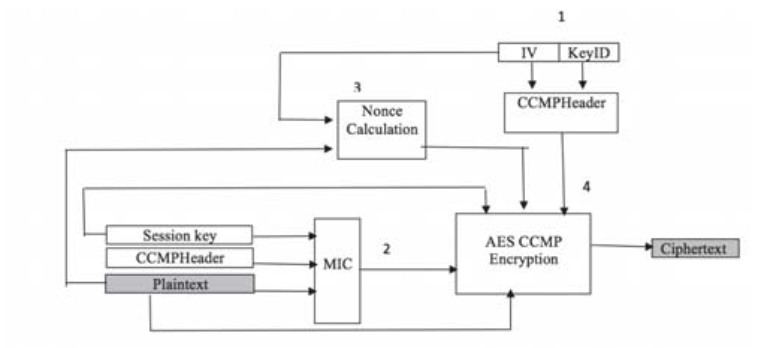
\includegraphics[scale=0.3]{images/ccmp.png}
	\caption{AES-CCMP operation}
	\label{fig:ccmp}
\end{figure}

\subsection{WPA2 advantages}
